%\section{Physical Human Factors Report: Tristan Griffith}
\rhead{\today}
\begin{center}
{\textbf{\Large Brief on Modal EEG Fingerprinting}}\\
\vspace{2mm}
{\large  Tristan Griffith}\\
\vspace{2mm}
{\large Dr. James Hubbard Jr.}
\noindent\rule{\textwidth}{2pt}
\end{center}

%\begin{wrapfigure}{r}{0.45\textwidth}
%\centering
%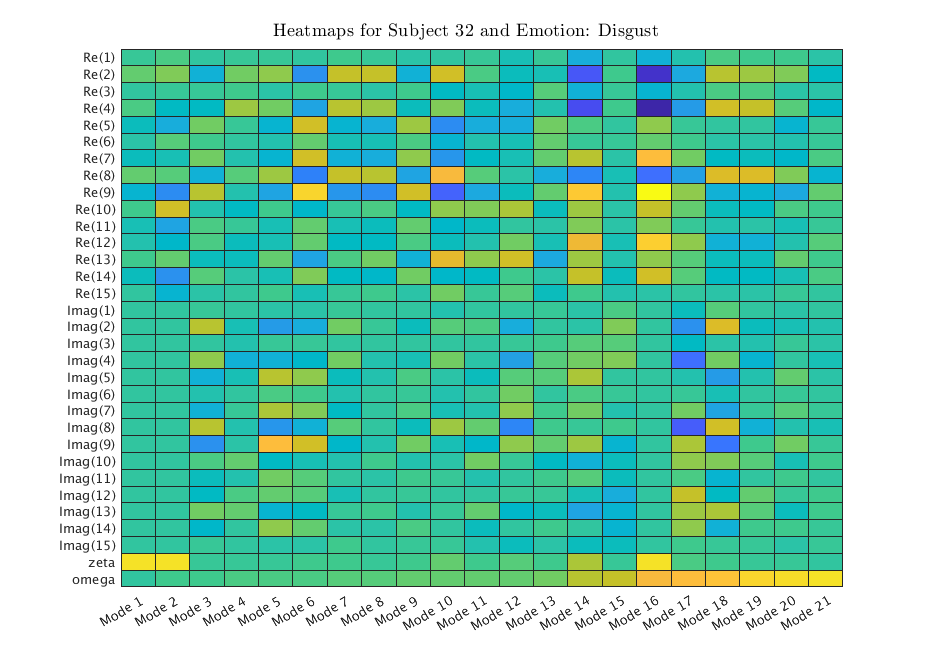
\includegraphics[scale=.3]{../../../figures/demo_map.png} 
%\caption{Modal Heatmap for Subject 32}
%\end{wrapfigure}
We postulate that data driven system identification methods of EEG data, such as Output Only Modal Analysis and Dynamic Mode Decomposition, may yield predictive models of cognition for more complete information flow between human operators and co-robots. As an initial step to verify that there is statistically significant information in these modal representations, an artificial neural network is proposed to discriminate subjects in a database. If the network shows sufficient accuracy in identifying subjects from the modal representation of their brain activity, we gain confidence that the modal representation is capturing significant information in the modes. It is shown that the network can discriminate 32 subjects from one another with $>$99\% accuracy based on knowledge of the significant modes alone.\


Output Only Modal Analysis (OMA) algorithms have been in use since at least the 90's. Originally developed for large mechanical structures, which are extremely difficult to precisely excite, OMA algorithms assume broadband stochastic input to the system in order to determine a state space model for a given system. The specific method applied to this data results from solving a set of linear equations with least squares to match data held in a Hankel matrix. When applied to the DEAP dataset, 21 significant complex modes are determined, which may be represented as a heatmap.\

\begin{wrapfigure}{r}{0.6\textwidth}
\centering
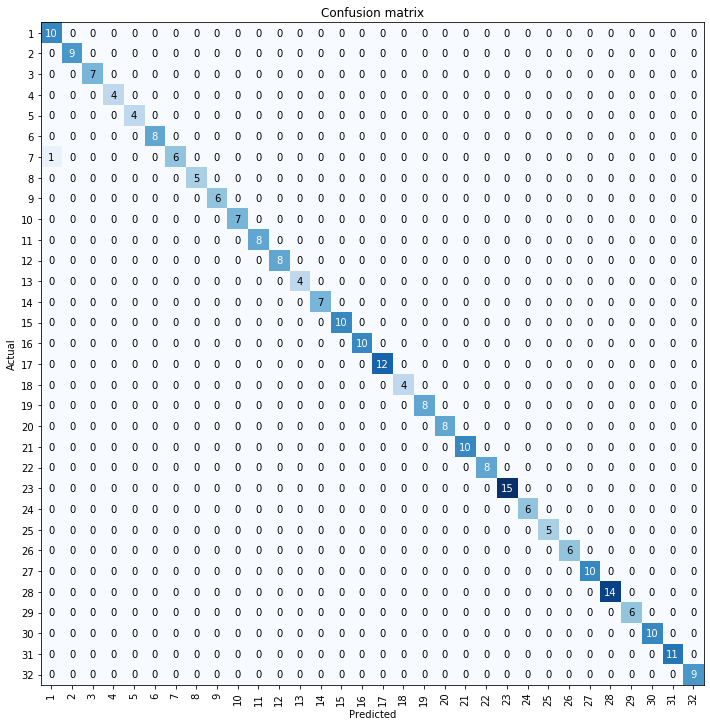
\includegraphics[scale=0.4]{../../../figures/conf_mat.png}  
\caption{Confusion Matrix for Neural Net}
\end{wrapfigure}
Having generated modal heatmaps for each of the 40 one minute trials across 32 subjects, 1280 modal heatmaps are generated. 1024 of these heatmaps are shown to the neural network, along with the subject label 1-32. The remaining 256 heatmaps are reserved for validation, without the subject label. Using a simple ResNet18 architecture, the network can distinguish subjects from unseen heatmaps with an accuracy of 99\% with less than 10 minutes of total training time. The relevant confusion matrix is included. Note that over all 256 unseen images, the network has only made one mistake, confusing subjects 1 and 7. This suggests that there is statistically significant information contained in the identified modes.




%\begin{displayquote}
%The class of monotone DNF expressions is learnable via an algorithm $B$ that uses $L=L(h,d)$ calls of examples and $dt$ calls of oracle, where $d$ is the degree of the DNF expression $f$ to be learnt and $t$ the number of variables.
%\end{displayquote}


%\begin{wrapfigure}{r}{0.55\textwidth}
%\centering
%\includegraphics[scale=.5]{../figures/complexity.png} 
%\caption{The Error-Complexity Trade Off}
%\end{wrapfigure}

